% withpage: ページ番号をつける (著者確認用)
% english: 英語原稿用フォーマット
\documentclass{ipsjprosym}
%\documentclass[withpage,english]{ipsjprosym}

\usepackage[dvips]{graphicx}
\usepackage{latexsym}

\begin{document}

% Title, Author %%%%%%%%%%%%%%%%%%%%%%%%%%%%%%%%%
\title{ATS言語を使って不変条件をAPIに強制する}

\affiliate{METASEPI}{METASEPI DESIGN}

\author{岡部 究}{Kiwamu Okabe}{METASEPI}[kiwamu@debian.or.jp]

\begin{abstract}
「モノのインターネット」という概念が提唱されています。バスケットボールのような、なんの変哲もないモノがインターネットに接続されるようになるでしょう。そのような機器は複雑な機能を持つ一方、現代の組み込み機器はC言語を用いて開発されており、不具合を誘発する危険性がつきまとっています。本論文ではこの問題に対する1つの解決策としてATS言語を紹介します。このATS言語はMLのような関数型言語で、静的な強い型を持ちます。また依存型を持ち、証明器としても機能します。さらにこの言語の線形型を使うことで、メモリやロックのようなリソースの制御を安全に行なうことができます。ATSコンパイラはC言語を経由して実行バイナリを生成するため、強い型による不変条件の強制は常にソースコードと同期しています。最後にわずか8kBのメモリしか持たないArduinoボード上でATS言語を使って設計したアプリケーションを動作させ、組み込み領域にATS言語を適用可能であることを示します。
% ``Internet of Things''; simple object such like basketball will be connected to the Internet. On the one hand such product should have many features, on the other various embedded system are designed with C language today. The C language code is possible to crash with various issues. In this paper, I introduce ATS language to address this issue. ATS language is a functional language such like ML, and has statically strong type system. It has dependent types and linear types that are used to manage memory resource and lock safely. The invariant captured by ATS's strong type is constantly synchronous the source code, because ATS compiler produces execution binary via C language. Finally, I show an ATS language application running on the Arduino board that only has 8kB SRAM, to proof that we can use ATS language for embedded system.
\end{abstract}

\begin{jkeyword}
ATS, 関数型言語, 依存型, 線形型, 組込開発
\end{jkeyword}

\maketitle

% Body %%%%%%%%%%%%%%%%%%%%%%%%%%%%%%%%%
\section{はじめに}

「モノのインターネット (IoT:Internet of Things)」という概念が提唱されています。バスケットボールのような、なんの変哲もないモノがマイクロチップを内蔵してインターネットに接続されるような世界を予想した概念がIoTです。そのIoTによる製造業への経済効果は2850億ドルと試算されています (ガートナー調べ \cite{iot_monoist})。このようなIoTデバイスに対する要件は以下のようなものになるでしょう。

\begin{itemize}
\item インターネットに接続可能なネットワークプロトコルを内蔵
\item 短時間/少工数による設計
\item 個人情報を保管/送信する機能
\item セキュリティへの配慮
\item ネットワーク非対応な機器よりもさらにインテリジェントな機能
\item 安価な価格を実現するため非力なハードウェアの使用
\end{itemize}

一方、現代の組み込み機器はC 言語やC++言語を用いて慎重に開発されています。しかしながら、これらの言語を使った開発では、バッファオーバーランに代表される数々の不具合が発生しやすくなります。これらの不具合発生を防ぐためにVDM \cite{vdm} やZ \cite{z_notation} のようなモデルベースの形式手法が用いられていますが、検証された形式モデルのC言語やC++言語のコードへの反映は人手で行う必要があります。したがって、製品の設計を更新するたびに形式モデルを製品のソースコードに同期させる工数が発生することになります。

この慎重な開発はPOSIX API上でのアプリケーション開発と比較にならないほどの工数を必要とします。にもかかわず、IoTデバイスはそのような開発者にPOSIX上のアプリケーションレベルの機能を要求します。このC言語を中心とした開発プロセスは今後持続可能なものなのでしょうか?ソフトウェア科学/工学はこの問題に対して、有効な手を打てないのでしょうか?

本論文ではこの問題に対するソフトウェア科学/工学の観点からの1つの解決策としてATS言語 \cite{ats} を紹介します。このATS言語はMLのような関数型言語で、静的な強い型を持ちます。またこの言語は依存型を持ち、Coq \cite{Coq_manual} のような証明器としても機能します。さらにこの言語の線形型を使うことで、メモリやロックのようなリソースの制御を安全に行なうことができます。ATS言語はC言語を経由して実行バイナリを生成するため、強い型による不変条件の強制は常にソースコードと同期しています。そのため製品のバージョンを数年にわたって更新する場合でも型とソースコードは機械的に同期されます。最後にわずか8kBのメモリしか持たないArduino Mega 2560ボード \cite{arduino-mega} 上でATS言語を使って設計したアプリケーションを動作させ、ATS言語が生成したC言語ソースコードが組み込み領域に実際に応用するにあたって十分な品質を持っていることを実証します。

\section{ATS言語とは}

ATS言語は、依存型を持つ関数型言語であるDependent ML \cite{Dependent-ML-Thesis} の後継にあたり、ボストン大学のHongwei Xiによって開発されています。

\begin{figure}[h]
\centering
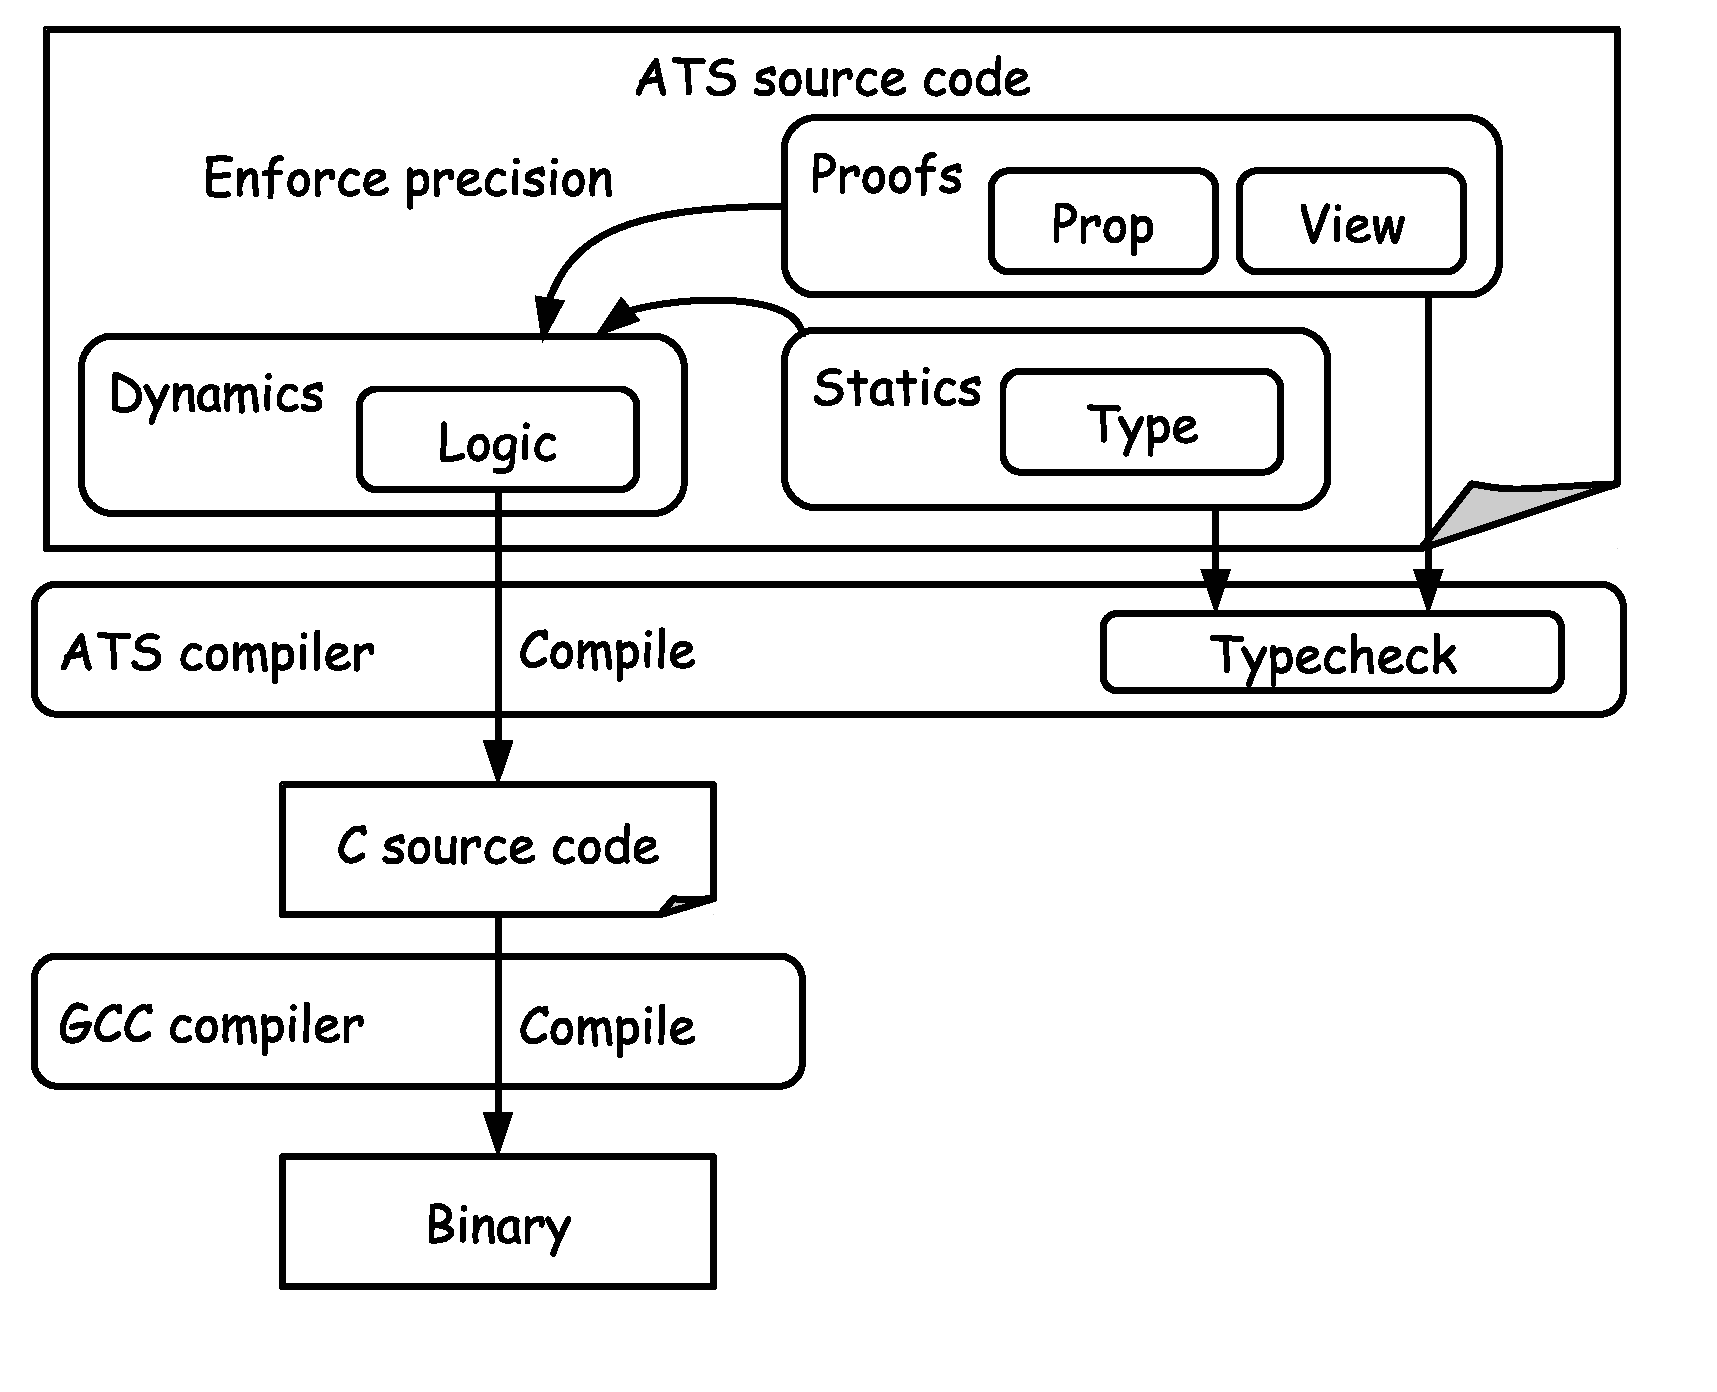
\includegraphics[width=75mm]{draw/flow.eps}
\caption{ATS言語の構成要素とコンパイルフロー}
\label{fig:flow}
\end{figure}

ATS言語のプログラムは大きく3つの要素から成り立っています (図\ref{fig:flow})。 動的な世界(Dynamics)、静的な世界(Statics)、証明の世界(Proofs)です。 動的な世界は通常のプログラミング言語と同じ実際に実行されるロジックです。動的な世界はATSコンパイラによってC言語に変換され、GCCによって実行バイナリになります。 静的な世界はHaskellやOCamlのような型推論を持つ言語における型のことです。 静的な世界は実行時エラーを防ぐ目的で、型の力で動的な世界を制約します。 証明の世界は依存型と線形型に分類できます。 依存型はCoqのような証明器として使うことができ、動的な世界のロジックに証明を与えることができます。 線形型はリソースを取り扱うことができ、例えばGCに頼らない動的な世界によるメモリ領域の管理を安全に行なうことができます。 動的な世界はコンパイルされて実行バイナリになりましたが、静的な世界と証明の世界はATSによるコンパイル時に評価(型検査)され、実行バイナリにはなりません。 しかし、静的な世界と証明の世界の検査に失敗すると、動的な世界のコンパイルも中止されます。

\begin{figure}[h]
\centering
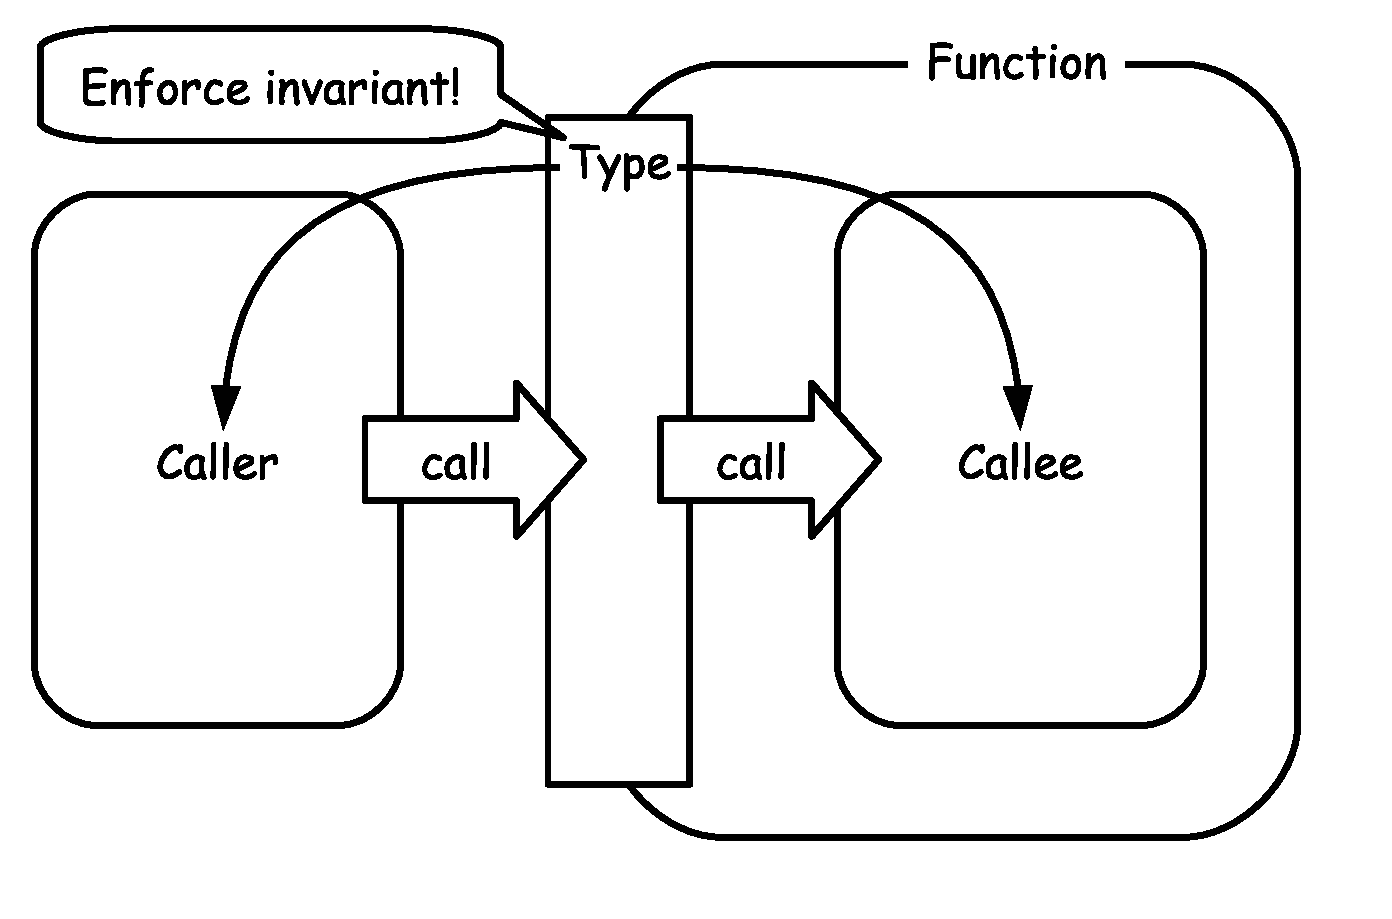
\includegraphics[width=75mm]{draw/enforce_invariant.eps}
\caption{型による制約の強制}
\label{fig:enforce_invariant}
\end{figure}

ATS言語ではインターフェイス宣言に依存型と線形型による強い制約をつけることができます (図\ref{fig:enforce_invariant})。通常の言語ではこのような制約はAPIの呼び出し元にのみ強制されますが、ATS言語では型推論によって、関数の呼び出し元と呼び出し先の双方に型による制約を与えることができます。

\section{ATSの型について}

ATS言語の型は依存型と線形型をそなえています。しかし、実行可能な言語においてこれらの強力な型を用いるイメージが想像しにくいかもしれません。そこで、本章では線形型を使ったリスト(線形リスト)を例にして、ATS言語の型の実例を解説します。

\begin{figure}[h]
\centering
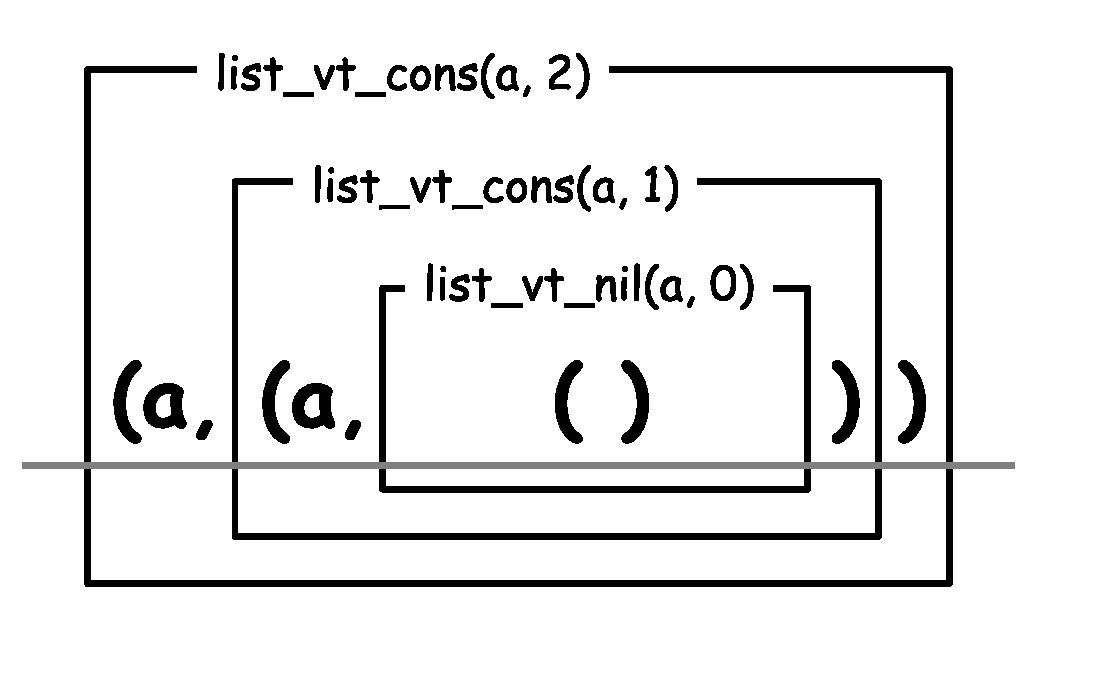
\includegraphics[width=50mm]{draw/list_vt_type.eps}
\caption{線形リストの型と構造}
\label{fig:list_vt_type}
\end{figure}

図\ref{fig:list_vt_type}に線形リストの型と構造を図示します。線形リストの動的なデータ構造はLISPのような通常のリストそのものです。しかし静的な型表現がこの動的なデータ構造に強制されています。ATS言語の基盤ライブラリであるpreludeでは以下のように線形リストの型を宣言しています。

\vspace{3mm}
\begin{verbatim}
(* ファイル: prelude/SATS/list_vt.sats *)
datavtype
list_vt0ype_int_vtype (a:vt@ype+, int) =
  | {n:int | n >= 0}
    list_vt_cons (a, n+1) of
      (a, list_vt0ype_int_vtype (a, n))
  | list_vt_nil (a, 0) of ()
stadef list_vt = list_vt0ype_int_vtype
vtypedef
List_vt (a:vt0p) = [n:int] list_vt (a, n)
\end{verbatim}
\vspace{3mm}

先のLISPのようなリスト構造はリストの長さ情報を持っていません。ところが、この線形リストは静的な型(依存型)によって長さを保持しています。$\{n:int | n >= 0\}$ の宣言は全称量化を使って静的な変数 $n$ を導入しています。この $n$ は $0$ 以上であるべきであるという制約も同時に宣言されています。さらに線形リストの終端ではこの静的な値は $0$ に固定されています。すなわちこの静的な値 $n$ は線形リストの長さを表現していることになります。この静的な値はコンパイル時まで存在していて、実機で動作する実行バイナリには含まれないことに注意してください。ATS言語はどのような動的な型表現も持ちません。静的な型表現のみを扱います。

datavtype宣言は線形型のデータ宣言です。そのため、このリスト構造は生産と消費という概念を持っています。生産しないかぎり、そのデータ構造をさわることはできません。また生産されたデータ構造は静的な文脈が終了するまでの間に消費されなければなりません。これらの制約をプログラムが破った場合にはコンパイル時エラーとなります。

この線形リストを使った関数群をいくつか見てみましょう。list\_vt\_make\_pair関数(図\ref{fig:list_vt_make_pair})は2つの要素x1とx2を引数に取り、線形リストの型list\_vtを返します。この関数はlist\_vt型を生産することが型宣言からわかります。このlist\_vt型はこれ以降のコードのどこかで消費しなければなりません。消費し忘れた場合にはコンパイル時エラーとなります。

\vspace{3mm}
\begin{verbatim}
fun{x:vt0p}
list_vt_make_pair (x1: x, x2: x):
                     <!wrt> list_vt (x, 2)
\end{verbatim}
\vspace{3mm}

\begin{figure}[h]
\centering
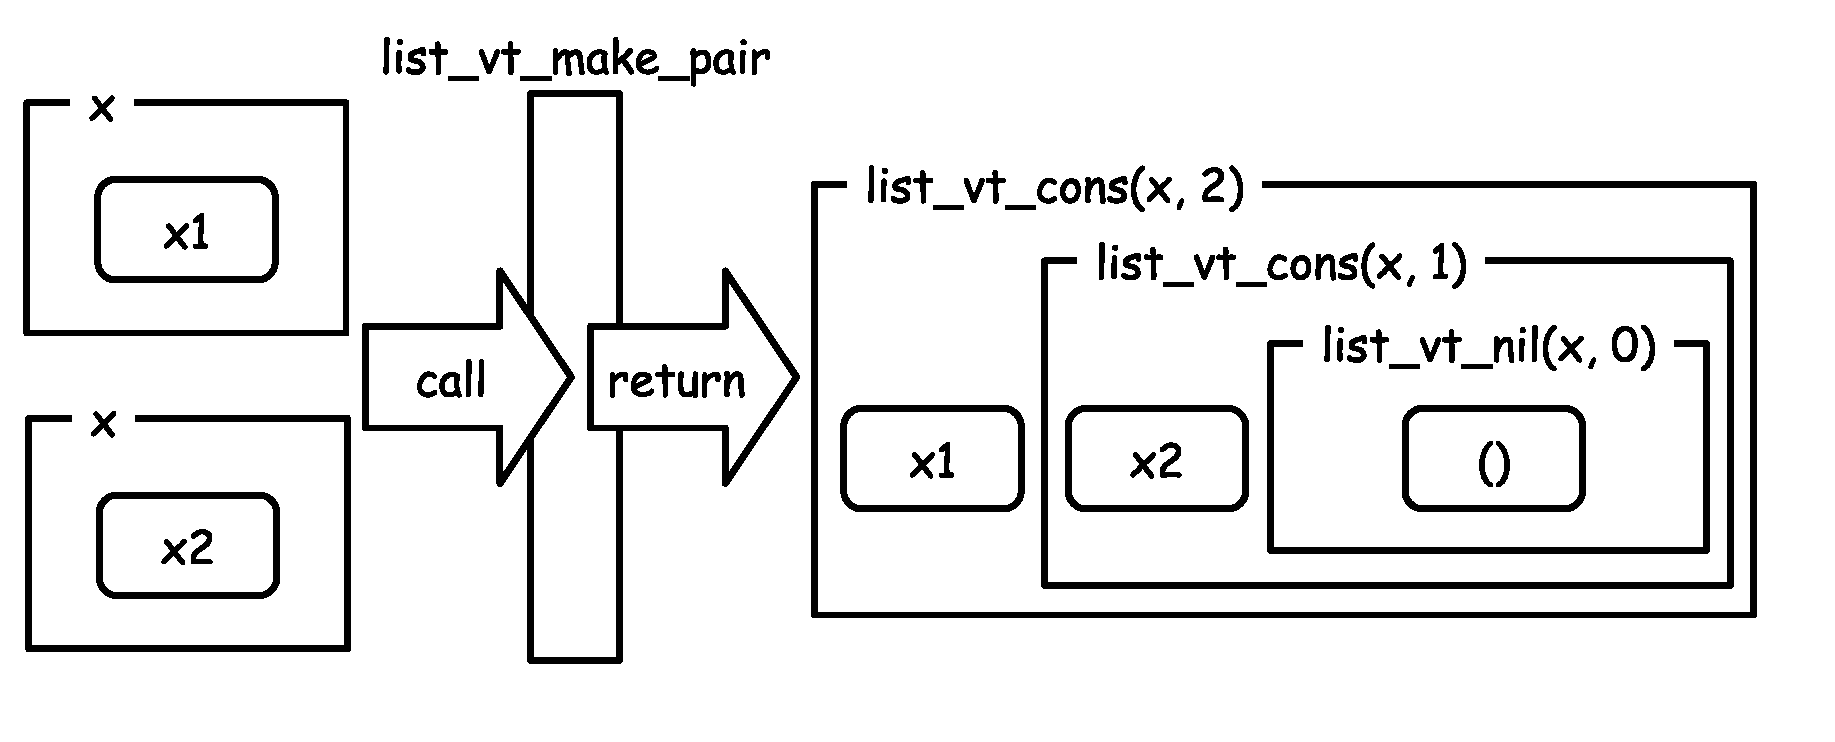
\includegraphics[width=75mm]{draw/list_vt_make_pair.eps}
\caption{2つの要素をペアにして線形リストを作る}
\label{fig:list_vt_make_pair}
\end{figure}

では生成された線形リストはどのように消費(すなわちそのメモリ領域を解放)すれば良いのでしょうか?それは単にfree関数を呼び出すだけです。このfree関数は多種の関数実体によってオーバーロードされており、線形リストの場合にはlist\_vt\_free関数(図\ref{fig:list_vt_free})が呼び出されます。ソースコードに付けられた型からもList\_vt型を受けとりvoid型を返す、つまりList\_vt型を消費していることがわかります。このList\_vt型が保持していたはずのメモリリソースを安全に解放することはATS言語の動的な部分の実装の責務です。つまりこのインターフェイスでは「線形リスト型の消費」は線形型による静的な検査の対象であり、「線形リストが保持していたメモリ領域の解放」は動的なコードの責務です。プログラマはこの2つが同じ意味になるように設計を行なうことで、動的なコードの挙動の中に静的な意味論を見出すことが可能になります。動的な意味論をコンパイル時に扱うことは多くの困難がありますが、静的な意味論はコンパイル時の型検査によってコンパイル時エラーとして扱うことができるのです。すなわち、ここでの「静的な意味論」とはまさに動的なプログラムの持つ「不変条件」に他なりません。

\vspace{3mm}
\begin{verbatim}
fun{x:t0p}
list_vt_free (xs: List_vt (INV(x))):
                            <!wrt> void
overload free with list_vt_free
\end{verbatim}
\vspace{3mm}

\begin{figure}[h]
\centering
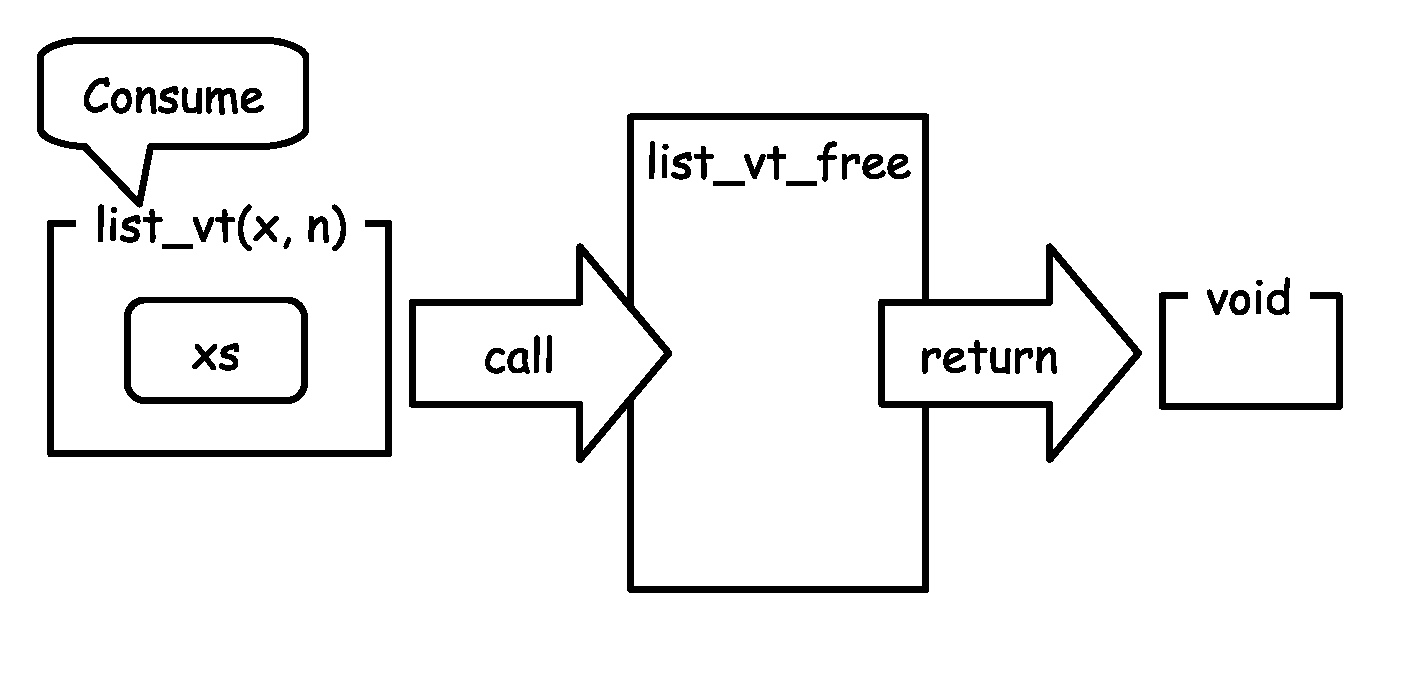
\includegraphics[width=75mm]{draw/list_vt_free.eps}
\caption{線形リストを解放する}
\label{fig:list_vt_free}
\end{figure}


次に線形リストをappendする関数であるlist\_vt\_append関数(図\ref{fig:list_vt_append})を見てみましょう。この関数は2つの線形リストxs1とxs2を取り、1つのappendされた線形リストを返します。この2つの線形リストxs1とxs2は消費されます。そしてappendされた線形リストが生産されます。以下のソースコードでappendされた線形リストに $n1+n2$ という依存型の制約がついていることがわかります。$\{n1,n2:int\}$ という静的な変数が全称量化によって導入されています。この2つの変数ははそれぞれxs1とxs2の線形リストの長さを表わしています。つまりappendされた線形リストの長さが $n1+n2$ であることを依存型を使って制約しています。この型はlist\_vt\_append関数の呼び出し元にも制約を強制しますが、呼び出し先であるlist\_vt\_append関数の実装にも制約を強制します。この制約をプログラマが破った場合にはコンパイル時エラーとなります。

\vspace{3mm}
\begin{verbatim}
fun{
a:vt0p
} list_vt_append
  {n1,n2:int} (
  xs1: list_vt (INV(a), n1),
  xs2: list_vt (a, n2)
) :<!wrt> list_vt (a, n1+n2)
\end{verbatim}
\vspace{3mm}

\begin{figure}[h]
\centering
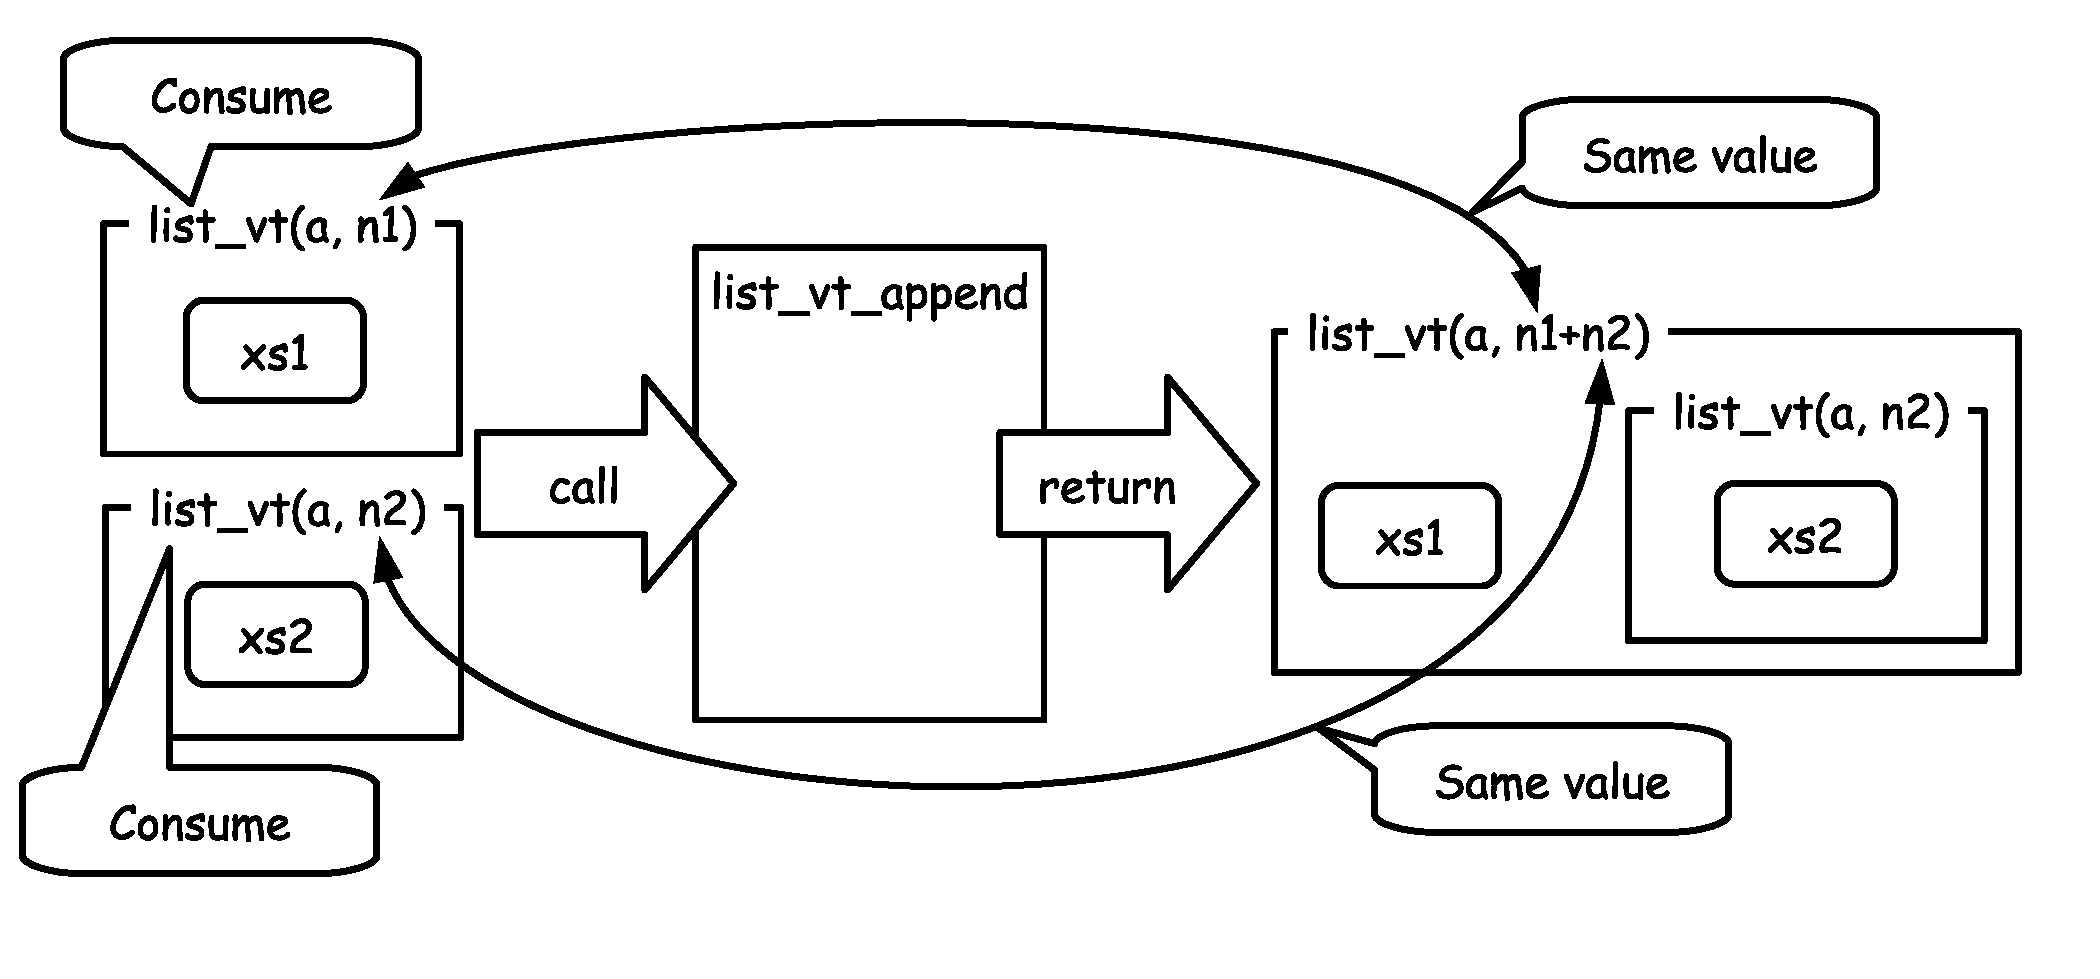
\includegraphics[width=75mm]{draw/list_vt_append.eps}
\caption{線形リストのappend}
\label{fig:list_vt_append}
\end{figure}

また、線形リストは $[]$ を使って添字指定で要素を読み出すこともできます。この $[]$ もまたオーバーロードされた関数で、その関数実体は渡される型によって異なります。線形リストの場合にはその実体はlist\_vt\_get\_at関数(図\ref{fig:list_vt_get_at})です。この関数にも全称量化 $\{n:int\}$ が導入されており、それは添字アクセスされる線形リストの長さを表わし、添字アクセスするインデックスがその線形リストの長さより小さくなければならないことが依存型で宣言されています。すなわち線形リストの範囲外を添字アクセスしてしまう不具合をコンパイル時に予防できます。さらに線形リストの引数xsの型には $!$ マークが付記されています。このマークは続く線形型を消費しないことを表わします。つまり添字指定で線形リストの要素を読み出しても、その線形リストは消費されません。これは納得できるインターフェイスでしょう。またこの関数の利用者は関数内部で線形リストが使用していたメモリが解放されないことを信じることができます。

\vspace{3mm}
\begin{verbatim}
fun{x:t0p}
list_vt_get_at{n:int}
  (xs: !list_vt (INV(x), n),
   i: natLt n):<> x
overload [] with list_vt_get_at
\end{verbatim}
\vspace{3mm}

\begin{figure}[h]
\centering
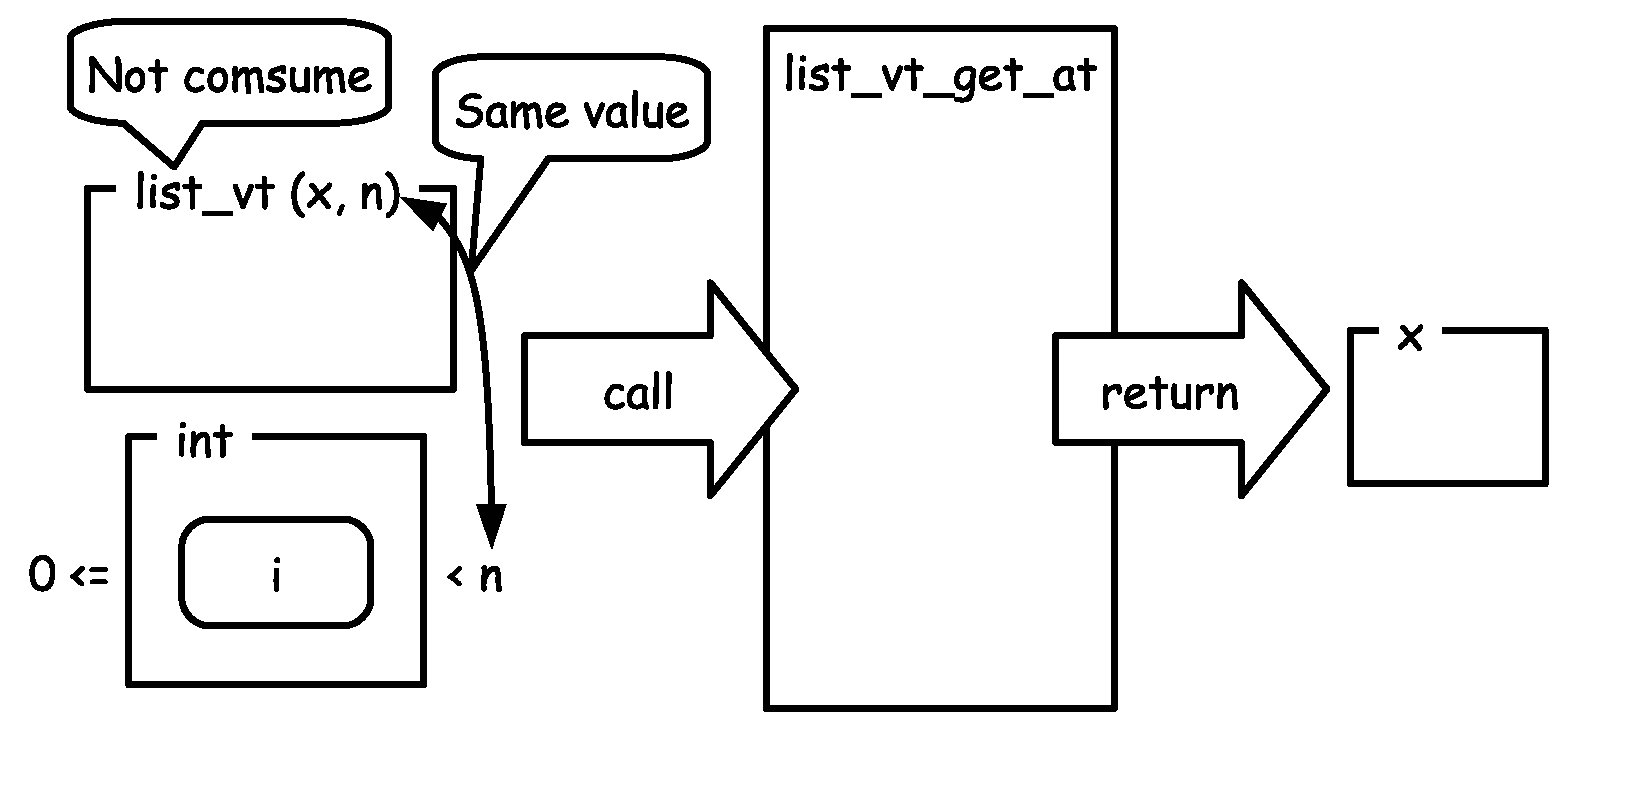
\includegraphics[width=75mm]{draw/list_vt_get_at.eps}
\caption{線形リストの添字指定}
\label{fig:list_vt_get_at}
\end{figure}

最後に線形リストのreverseであるlist\_vt\_reverse関数(図\ref{fig:list_vt_reverse})を見てみましょう。この関数は、引数であるxsを消費し、逆順にした新しい線形リストを生成します。全称量化による制約は「引数と返り値の線形リストの長さが同じ」ということだけ強制しています。そのためこの型では「線形リストの中身が本当に逆順になっているのか?」ということまでは強制できていないことがわかります。それでも、引数として渡された逆順になる前の線形リストは消費されているので、仮にlist\_vt\_reverse関数の実装がその線形リストのメモリ領域を逆順にした新しい線形リストのために再利用したとしても、元の線形リストは消費されているためにプログラマが誤って元の線形リストにアクセスする危険性を防止できます。

\vspace{3mm}
\begin{verbatim}
fun{x:vt0p}
list_vt_reverse{n:int}
  (xs: list_vt (INV(x), n)):
             <!wrt> list_vt (x, n)
\end{verbatim}
\vspace{3mm}

\begin{figure}[h]
\centering
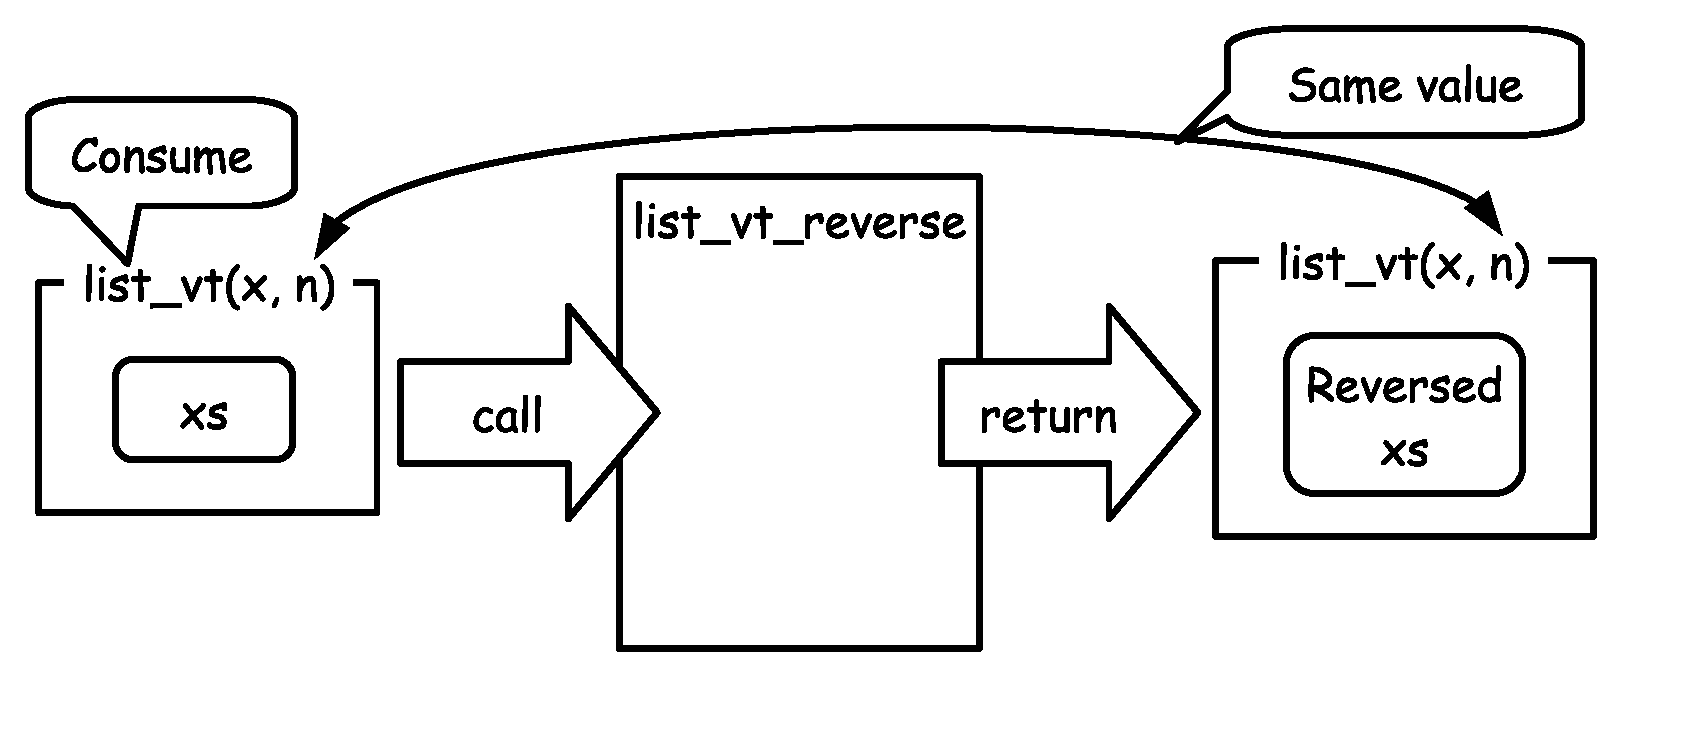
\includegraphics[width=75mm]{draw/list_vt_reverse.eps}
\caption{線形リストのreverse}
\label{fig:list_vt_reverse}
\end{figure}

\section{ArduinoにおけるATSプログラミング}

ATS言語による組み込み開発の適正を評価するために、Arduino Mega 2560ボード上で動作するアプリケーションをATS言語で試作しました。このボードは以下のような仕様です。

\vspace{3mm}
\begin{description}
  \item[Architecture] 8-bit Harvard architecture
  \item[Microcontroller] ATmega2560
  \item[Flash Memory] 256kB
  \item[SRAM] 8kB
  \item[Clock Speed] 16MHz
\end{description}
\vspace{3mm}

本稿を執筆している段階では、さらにメモリの少ないArduino Unoボード \cite{arduino-uno} 上でも同様のアプリケーションの動作に成功しています。このアプリケーションのソースコードは \cite{arduino-ats} から入手可能です。

\begin{figure}[h]
\centering
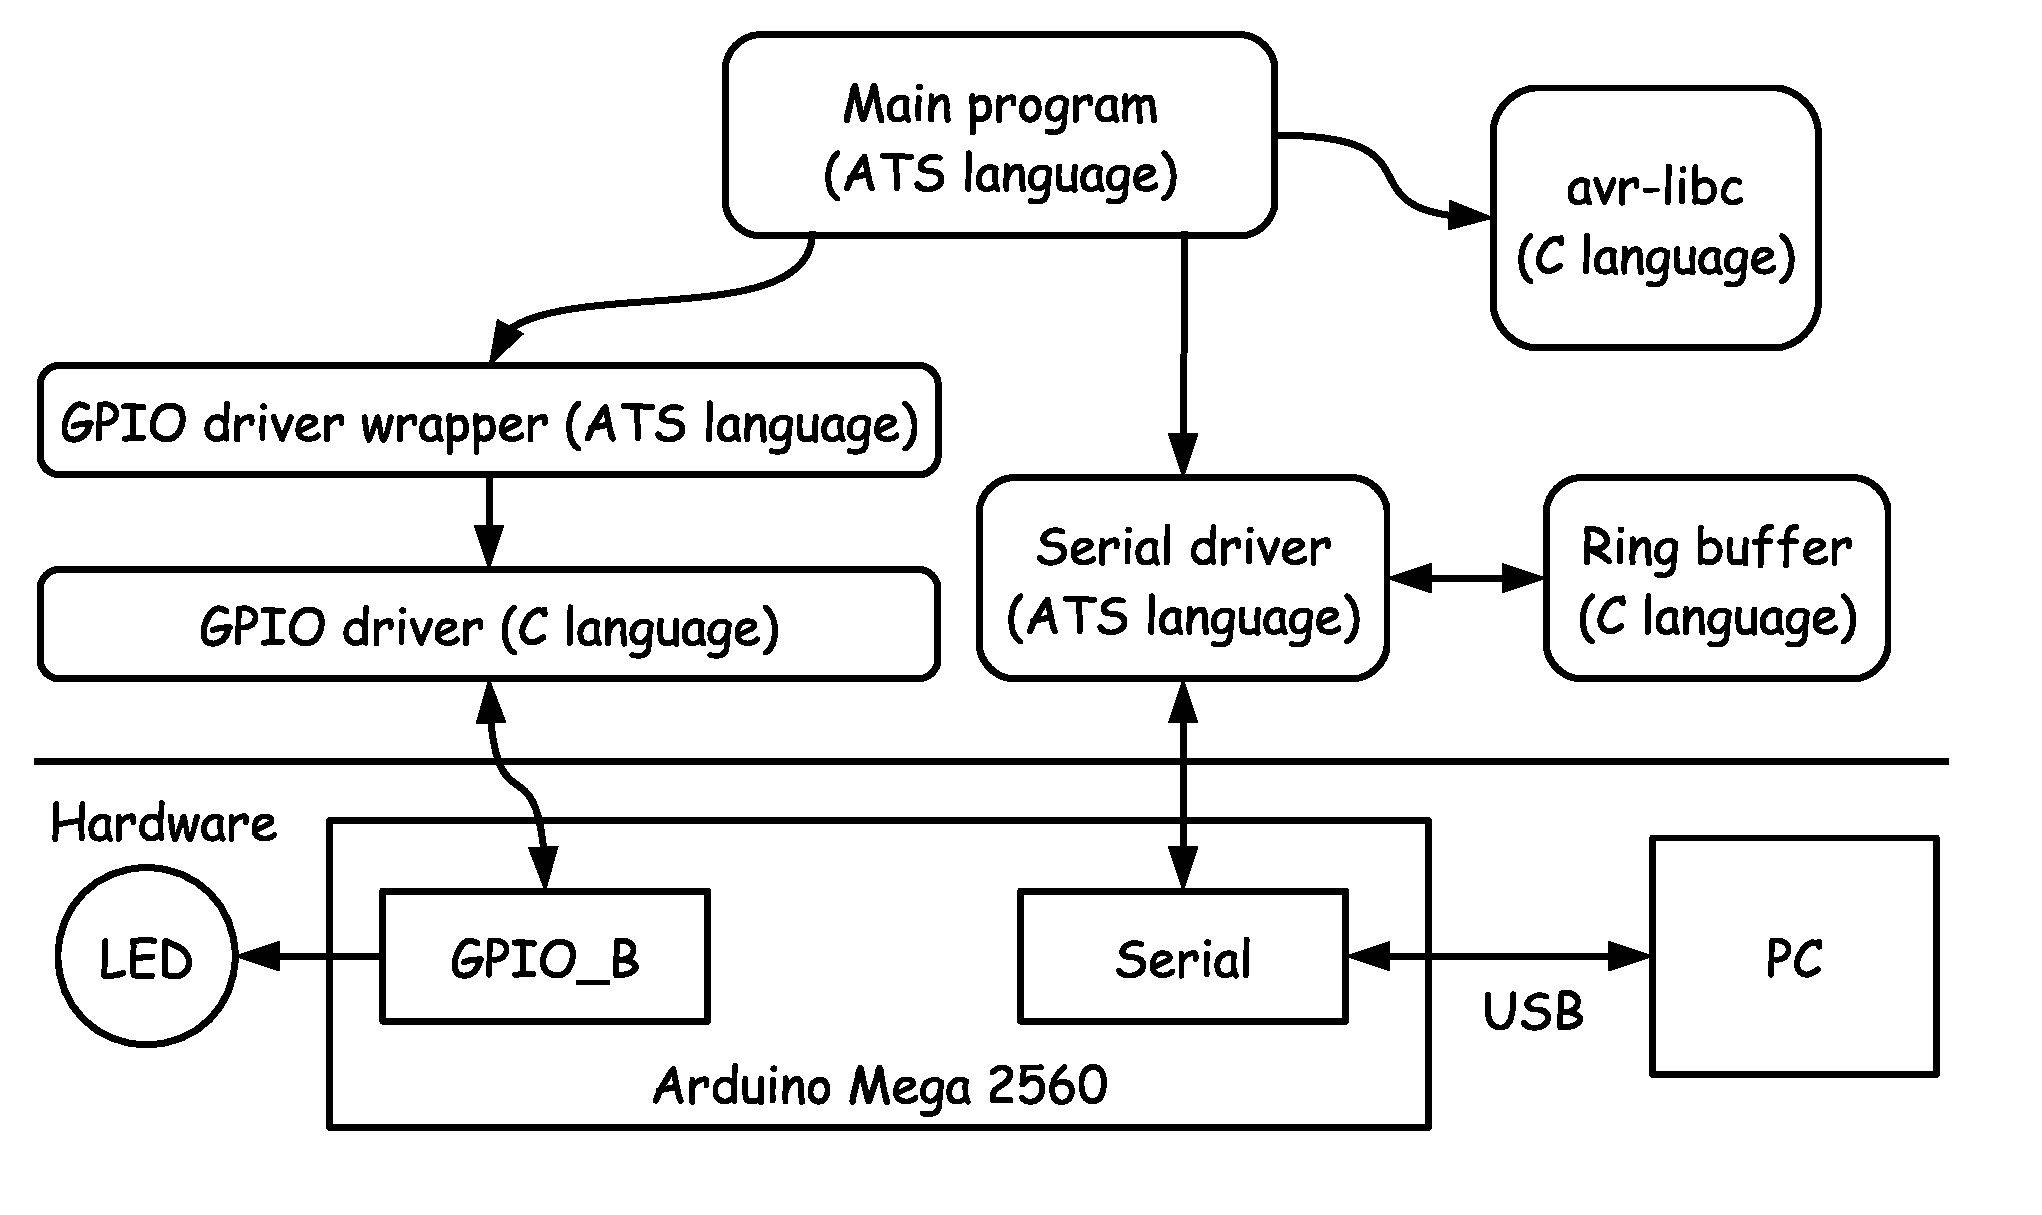
\includegraphics[width=75mm]{draw/demo_ats_arduino.eps}
\caption{Arduino上におけるATSアプリケーション例}
\label{fig:demo_ats_arduino}
\end{figure}

本アプリケーションのソフトウェアアーキティクチャは図\ref{fig:demo_ats_arduino}のようになります。本アプリケーションはハードウェアの機能としてGPIOとシリアルポートを使用します。GPIOはArduinoのGPIOライブラリを経由してATS言語から使用します。シリアルポートのレジスタ群にはATS言語から直接さわります。ただし、シリアルポートから読み書きするデータを一時保管するリングバッファについてはArduinoライブラリを流用することにしました。この2つの抽象化によって、どのようなOSのサポートなしに、さらにGCやmallocヒープさえ準備せずにATS言語を使ってアプリケーションを書くことができます。

なぜGCとmallocヒープなしに強い型を用いた関数型プログラミングを行なうことが可能なのでしょうか?それはATS言語が値渡し(call-by-value)をコアにしていることと、線形型を使ったメモリリソースの管理によって実現されています。線形型を使うことで固定領域のメモリを安全に使用することが可能になり、さらにその領域外へのアクセスをメモリ領域のサイズに依存した依存型を使って防止することも可能です。

\section{ATSによる組込開発手法の考察}

前章でATS言語を使ってOS不在の領域における組み込み開発が可能なことを示しました。本章ではATS言語を用いた組み込み開発の利点と欠点についてまとめます。

その利点は静的な強い型と依存型、線形型をOSなしに利用することができることです。これまでこのような型による制約はPOSIX APIのようなインターフェイスを下支えするOSなしには利用できませんでした。そのため組み込みにおける開発では、形式手法を用いた後付けによる制約強制の手法が盛んに用いられてきました。ATS言語を使えば、型による制約によって実機で動作させるソースコードに制約を付けることが可能になります。製品バージョンを重ねてソースコードが成長したとしても、この制約は機械的に引き継がれることになります。これは今までの形式手法とは全く異なるレベルの画期的な技術です。

一方、欠点もあります。GCを持つHaskellやOCamlのような関数型言語と比較すると、GCを使わずに線形型を用いるATSプログラミングは他のプログラミング言語には見られない特殊な設計能力が要求されます。近年、線形型を使用可能な言語としてRust言語 \cite{rust} も人気ですが、Rust言語は純粋な線形型をではなくポインタに限定して線形型を用います。著者もHaskellとOCamlのプログラミング経験はありましたが、ATS言語の依存型と線形型に慣れるのにはかなりの時間が必要でした。現在組み込み開発の現場ではC言語とC++言語を使っているため、一般的な関数型言語とさらに加えてATS言語を習熟するのは容易ではないでしょう。

\section{結論と今後の課題}

ATS言語による強い型の強制がOSさえないような組み込みドメインに対して有用であることを述べました。しかし、ATS言語の力を普及させるためにはATS言語の教育プログラムが重要であることも考察しました。そこで筆者は2つのプロジェクトを推進しています。

1つ目は、Japan ATS User Group (JATS-UG) \cite{jats-ug} です。このプロジェクトではインターネット上で入手可能なATS言語に関する文献を日本語に随時翻訳しています。特に「ATSプログラミング入門 \cite{INT2PROGINATS-J}」は有用でしょう。本稿執筆時点ではこのドキュメントが最も体系的にATS言語を解説しています。また、線形型に関しても本稿執筆時点では日本語で読める最も詳しいドキュメントでしょう。またATS言語の型システムを理論的に解説した論文``Applied Type System (Extended Abstract)'' \cite{ATStypes03} も日本語訳しています。詳細は先のJATS-UGのWebページをご覧ください。

2つ目は、Functional IoT \cite{fpiot} です。このプロジェクトでは8-bit AVRと16-bit MSP430、32-bit ARM Cortex-Mシリーズの3つのアーキティクチャを対象として、ATS言語のような強い静的な型を持つ言語を使ったマイコンプログラミングを試行しています。このプロジェクトにはさらに2つの目的があります。1つ目はこのプロジェクトを通してATS言語のような組み込み領域に適用可能なプログラミング言語をサーベイすること。2つ目は製品よりも小さな領域の関数型組み込みプログラミングを通じて、そのデザインパターンを蓄積することです。日本のみならず世界を見わたしてもこの規模のアーキティクチャ上で動作する関数型プログラミングの実例はほとんどありません。そのため依存型や線形型をどのように駆使すべきであるのか、そのイディオムが圧倒的に不足しています。

最後に、先の論文``Applied Type System''は2004年に発行されています。しかしATS言語の作者であるHongwei Xiの知るかぎりでは、この型システムの実用例はATS言語のみであるそうです。関数型言語の持つ安全性がOSの外の領域でも活用できるために、このApplied Type Systemのさらに先にある理論の探求がさかんに行なわれることを願ってやみません。

\begin{acknowledgment}
ATS言語に関して助言をくれたボストン大学の准教授であるHongwei XiとATSコミュニティに感謝します。
\end{acknowledgment}

\begin{QandA}
\item[A] 線形型にvalで別名を作るとどうなるのですか?
\item[岡部] 消費されます。以下に例を付記します。

\begin{verbatim}
(* コンパイルNG: let valでも線形型が消費されてしまう *)
#include "share/atspre_staload.hats"
implement main0 () = {
  val l1 = list_vt_make_pair<int> (1, 2)
  val l2 = l1
  val () = let val l3 = l2
           in println! l3 end
  val () = free l2
}

(* コンパイルOK: valで線形型が消費される *)
#include "share/atspre_staload.hats"
implement main0 () = {
  val l1 = list_vt_make_pair<int> (1, 2)
  val l2 = l1
  val () = println! l2
  val () = free l2
}
\end{verbatim}

\item[B] リングバッファをATSで書くのは難しいのですか?
\item[岡部] 公式ドキュメントに例があるぐらいなので、リングバッファ自体は簡単です。しかし、スレッドセーフ化や再入可能にするのはそれなりに難しいと思います。
\item[C] ATS言語でマルチスレッドを生かしたプログラミングをするにはどうすれば良いのですか?
\item[岡部] セッションのようなものを作ることになります。例えばmutexのロックと開放では、その間にセッションが存在すると考えることができます。セッションの間は静的な型を効果的に使うことができます。
\item[D] ATSに辿りつくまでのMetasepiプロジェクトの歴史について簡単に説明してください。
\item[岡部] ATSを使ったイテレーションは2番目です。1番目ではHaskell言語とjhcコンパイラを使っていました。Haskell言語の欠点は、メモリ領域の扱いがルーズであることと、マシン表現と言語表現にギャップがあることです。一方ATS言語の欠点は、抽象化の機能がHaskell言語と比較して弱いことです。
\end{QandA}

% BibTeX を使用する場合 %%%%%%%%%%%%%%%%%%%%%%%%%%%%%%%%%
\bibliographystyle{ipsjsort}
\bibliography{../bibtex/reference,../bibtex/jreference}

\end{document}
